\chapter{Implementierung}
\label{sec:imp}

Im Folgenden werden einige interessante Gesichtspunkte der Implementierung, die in
Kapitel\,\ref{sec:draft} nur kurz angesprochen wurden, genauer herausgearbeitet.

\section{Layout}
\label{sec:layout}

\begin{figure}[ht]
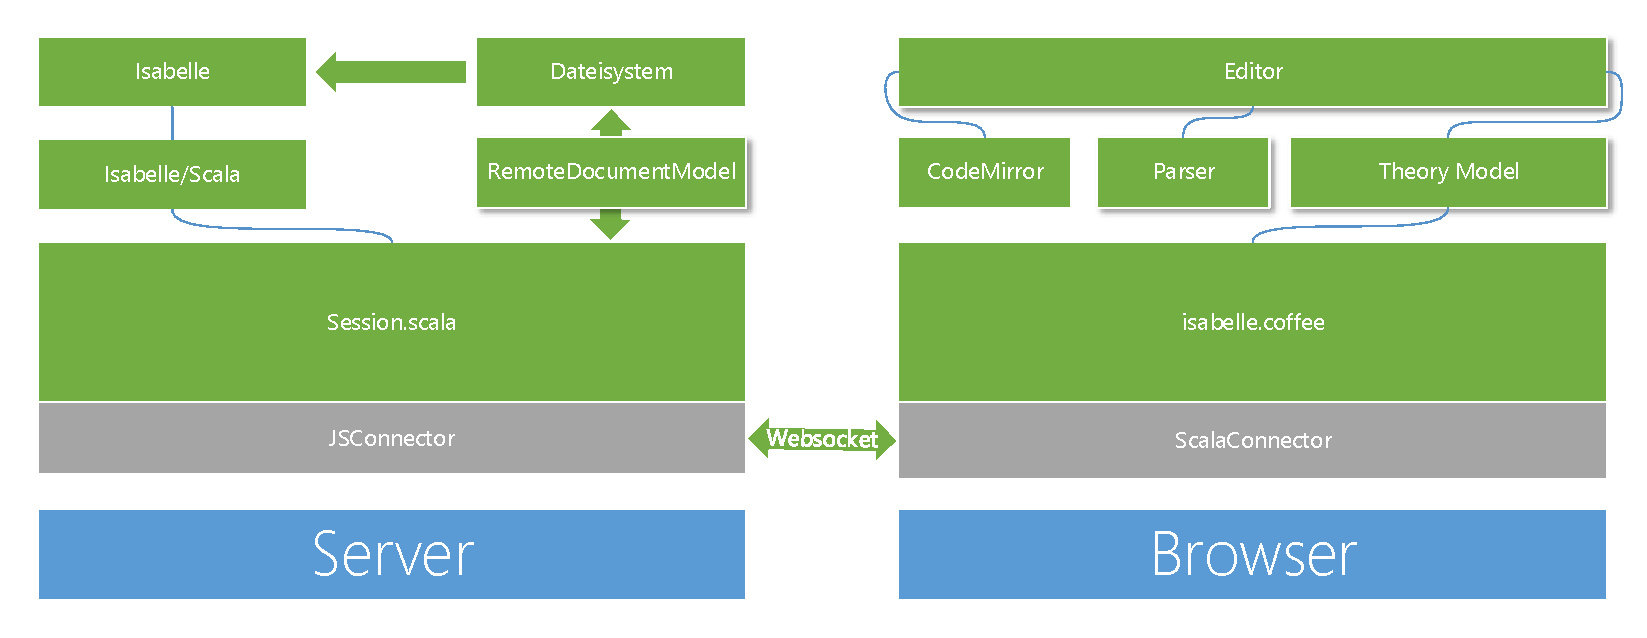
\includegraphics[width=\linewidth]{images/layout}
  \caption{Architekturlayout}
  \label{fig:layout}
\end{figure}

Abbildung\,\ref{fig:layout} zeigt ein grobes Architekturlayout. Server und Browser kommunizieren
über die serverseitige Schnittstelle \texttt{JSConnector} bzw. clientseitig über den
\texttt{ScalaConnector} (Abschnitt\,\ref{sec:jsc}). Die verknüpften Objekte sind dabei
\texttt{Session} aus \texttt{Session.scala}, wovon für jede Clientseitige Sitzung eine Instanz
besteht sowie im Browser das Objekt \texttt{Session} aus \texttt{isabelle.coffee}.

Im Browser wird ein Modell aller Theorien verwaltet, welches sowohl von der \texttt{Session} (z.B.
Serverseitiges Syntax-Highlighting in Abschnitt\,\ref{sec:ssyntax}), als auch vom Editor verändert
werden kann. Die Kommunikation erfolgt über eventbasierte Callbacks. Jeder \texttt{Editor} erzeugt
eine angepasste \texttt{CodeMirror} Instanz zur Visualisierung mit einem Parser, welcher die äußere
Syntax erkennt und direkt in die Darstellung integriert (Abschnitt\,\ref{sec:syntax}).

Auf dem Server wird das \texttt{RemoteDocumentModel} mit den \texttt{LineBuffer}n (Siehe
Abschnitt\,\ref{sec:linebuffer}) verwendet, um den Zustand der Theorien synchron zum Client zu
verwalten.

\section{Abstraktion vom Protokoll}
\label{sec:jsc}

Um das Protokoll austauschbar zu gestalten, wurde eine Abstraktion über WebSockets implementiert.
Hierfür wurde seitens des Browsers der \texttt{ScalaConnector} und serverseitig der
\texttt{JSConnector} entwickelt.

\subsection{ScalaConnector}

Das \texttt{ScalaConnector} wurde in CoffeeScript als RequireJS-Modul implementiert und dient zur
Kommunikation mit dem Webserver. Ein beliebiges Objekt kann sich über den ScalaConnector mit dem
Server verbinden, sodass dieser dann direkt die Funktionen dieses Objekts aufrufen kann.

\begin{lstlisting}[language=coffee]
define -> class ScalaConnector
  constructor: (@url,@object,init) -> ...
\end{lstlisting}

Dem Konstruktor wird zum einen die url (\texttt{url}) des WebSockets mit dem verbunden werden soll,
zum anderen das Objekt (\texttt{object}), welches dem Server als Schnittstelle zur Verfügung
gestellt werden soll übergeben. Als optionales Argument kann eine \texttt{init}-Funktion übergeben
werden, welche aufgerufen wird, sobald die Verbindung hergestellt worden ist.

Intern wird im Konstruktor zunächst eine Verbindung aufgebaut und an das
\texttt{onmessage}-Callback des WebSockets verbunden:

\begin{lstlisting}[language=coffee]
@socket = new WebSocket(@url) # Connect to server
@socket.onmessage = (e) =>    
  @bytesDown += e.data.length # Downstream traffic measure
  recieve(JSON.parse(e.data)) # Interpret messages as JSON
\end{lstlisting}

Die \texttt{recieve}-Funktion unterscheidet hierbei zwischen Antworten auf eigene Anfragen und
Anfragen bzw. Kommandos vom Server:

\begin{lstlisting}[language=coffee]
recieve = (e) =>  
  if e.action # if an action is defined this is a command from the server
    f = @object[e.action] # we try to find the action on the connected object
    if f?
      result = f.apply(f,e.args) or null # execute the function and save the result
      # if an id for the message is defined the server awaits an answer with the result of the
      # function execution. otherwise this is just a command (or server-push)
      if e.id then @socket.send JSON.stringify 
        resultFor: e.id
        success: true
        data: result
    else # if the action does not exist we send an error message to the server
      if e.id then @socket.send JSON.stringify
        resultFor: e.id
        success: false
        message: "action '#{e.action}' does not exist"
      else console.error "action '#{e.action}' does not exist"
  else # if no action is defined the message must be an answer to a request
    callback = @results[e.resultFor] # retrieve the callback function for this action
    if callback 
      callback(e.data) # answer the callback
      @results[e.resultFor] = null # delete the callback function
\end{lstlisting}

Hierbei werden drei verschiedene Fälle unterschieden:

\begin{itemize}  
  \item Die Nachricht enthält das Feld \texttt{action}: Es handelt sich um eine
Anfrage oder ein Kommando vom Server.
  \begin{itemize}
    \item Wenn zusätzlich das Feld \texttt{id} definiert ist, erwartet der Server eine Antwort mit 
    dieser id als Referenz, es handelt sich also um eine Abfrage.
    \item Wenn das Feld nicht enthalten ist, handelt es sich um eine einfache Nachricht vom Server
    auf die nicht geantwortet wird.
  \end{itemize}
  \item Wenn die Nachricht das Feld \texttt{action} nicht enthält, handelt es sich um eine Antwort 
  auf eine vorherige Anfrage des Clients. In diesem Fall wird die entsprechende Callback-Funktion mit
  dem Ergebnis des Servers aufgerufen.
\end{itemize}

Der Vorteil der Repräsentation über fehlende Felder ist die Kompaktheit der Daten. Da der WebSocket
konfiguriert ist, die Daten zusätzlich komprimiert zu übertragen, sind die Nachrichten sehr klein.
Noch kleiner können sie gemacht werden, indem ein eigenes Protokoll implementiert wird. Diese
abstrakte Implementierung macht das sehr einfach, da nur an zwei Stellen etwas ausgetauscht werden
muss.

Das Gegenstück ist natürlich das Versenden von Daten. Antworten auf Serveranfragen werden wie oben
beschrieben automatisch verschickt. Anfragen können über die \texttt{call}-Funktion versendet
werden.

\begin{lstlisting}[language=coffee] 
    call: (options) =>      
      if options and options.action        
        if options.callback
          @results[@id] = options.callback
          options.id = @id
          @id += 1
        @socket.send JSON.stringify(options)
      else
        console.error 'no action defined'
\end{lstlisting}

Die Funktion erwartet ähnlich wie die \texttt{ajax}-Funktion aus jQuery ein Konfigurationsobjekt
\texttt{options}, in welchem mindestens das Feld \texttt{action} definiert sein muss. (Andernfalls
wird ein Fehler geworfen) Darüber wird definiert welche Funktion auf dem Server aufgerufen werden
soll.

Wenn zusätzlich das Feld \texttt{callback} mit einer Callback-Funktion belegt wird, wird eine
\texttt{id} generiert, welche dem Server gesendet wird um unter dieser \texttt{id} zu antworten
(Siehe oben). Das gesamte Objekt wird nun (natürlich ohne die Callback-Funktion) an den Server als
JSON übertragen. Wenn keine Callback-Funktion definiert wurde, wird auch keine Antwort vom Server
gesendet.

\subsection{JSConnector}

Das Pendant zum \texttt{ScalaConnector} auf der Serverseite ist der \texttt{JSConnector}. Dieser
wurde mit Hilfe dynamischer Typisierung verwirklicht und ist unter \texttt{/app/js/JSConnector} zu
finden.

Für die Kommunikation verwenden wir die Akka-Iteratees und Enumeratees (Siehe auch
Abschnitt\,\ref{sec:iteratees}). Iteratees werden dabei für den Eingehenden Datenstrom über den
Websocket und Enumeratees für die zu sendenden Daten verwendet. Da wir hier ein imperatives Modell
entwickeln wollen, können wir zur Erzeugung des Enumeratee auf die
\texttt{Concurrent.broadcast}-Funktion aus der Play API zurückgreifen (Für genauere Informationen
verweisen wir hier auf die Dokumentation in\,\cite{play})

\begin{lstlisting}
trait JSConnector {
  val (out, channel) = Concurrent.broadcast[JsValue]
  val in = Iteratee.foreach[JsValue] { json =>
    ...
\end{lstlisting}

Über den \texttt{channel} ist es später möglich, Nachrichten an den Client zu senden (welcher per
WebSocket an den Enumeratee \texttt{out} verbunden ist). Die eigentlich interessanten Punkte sind
jedoch wie beim Client das Empfangen sowie das Versenden von Nachrichten.

Beim Empfang wird genau wie im Browser zwischen den drei beschriebenen Fällen unterschieden:

\begin{lstlisting}
  val in = Iteratee.foreach[JsValue] { json =>    
    (json \ "action").asOpt[String] match {
      case Some(a) => // an action is defined    
        require(actions.isDefinedAt(a))
        // create a future for the action
        scala.concurrent.future(actions(a)(json \ "data")).onComplete {
          case Success(result) => // future succeeded
            (json \ "id").asOpt[Long].map(id => channel.push(Json.obj{
                "resultFor" -> JsNumber(id), // request id
                "data" -> js.convert(result), // result of invocation))
          case Failure(msg) => debug(msg) // future failed
           
        }
      // no action defined: this is a result message
      case None => (json \ "resultFor").asOpt[Long] match {
        case Some(id) => 
          val p: Promise[JsValue] = js.requests(id)
          if (!(json \ "success").as[Boolean]) // request failed
            p.failure(new Exception((json \ "message").as[String]))
          else // request succeeded
            p.complete(Try(json \ "data"))
          js.requests.remove(id)
        case None => debug('invalid message from websocket',json)
      }
    }
  }.mapDone(_ => onClose)
\end{lstlisting}

Um die Ausführung nicht zu blockieren, verwenden wir Futures (Abschnitt\,\ref{sec:futures}), die
Anfragen des Clients in eigenen Threads ausführen. Wenn der Client eine Anfrage stellt, wird der
entsprechenden Funktion das Datenobjekt aus dem empfangenen JSON-Code übergeben und diese in einem
Future ausgeführt. Wenn das Future die Ausführung erfolgreich beendet, wird das Ergebnis im
Bedarfsfall (\texttt{id} ist in der Anfrage definiert) an den Client zurückgesandt. Im Fehlerfall
wird das Ereignis geloggt. Weil Fehlerfälle für den Client uninteressant sind, da das Debugging auf
dem Server stattfinden soll, werden sie in diese Richtung nicht übertragen. Wenn signalisiert
werden soll, dass eine Aktion aus einem bestimmten Grund nicht ausgeführt werden kann, sollte mit
einem geeigneten Datentyp ein wohldefiniertes Ergebnis von der entsprechenden Funktion zurückgegeben
werden (z.B: \texttt{Option[T]}).

Zu beachten ist, dass für ein erfolgreiches Versenden das Funktionsergebnis einen Typ haben muss,
welcher die Typklasse \texttt{json.Writes} implementiert, damit die Daten konvertiert werden können.
Ist dies nicht der Fall, kann der Code nicht übersetzt werden, da ein Typfehler vorliegt.

Für die Kommunikation nach \glqq unten\grqq\ nutzen wir dynamische Typisierung. In einer Klasse, die
den \texttt{JsConnector} einmischt werden drei Objekte zur Verfügung gestellt:

\begin{itemize}
  \item \texttt{js.ignore} kann verwendet werden, um Kommandos oder Informationen an den Client zu 
  senden, ohne dass eine Antwort erwartet wird.
  \item Über \texttt{js.async} können Anfragen versendet werden, für die man ein Future erhält, 
  das bei Erhalt der Nachricht erfüllt wird.
  \item In manchen Fällen kann es notwendig sein, innerhalb eines Threads zu blockieren bis die 
  Antwort vom Browser erhalten wurde. Dafür kann \texttt{js.sync} verwendet werden.
\end{itemize}

Der Aufruf \texttt{js.async.moveCursor(4,1)} könnte beispielsweise dazu führen, dass folgendes JSON-
Objekt an den Browser gesendet wird:

\begin{lstlisting}
{
  action: "moveCursor",
  id: 12803,
  data: [4,1]
}
\end{lstlisting}

Auf dem Client würde dadurch die Funktion \texttt{moveCursor} mit den beiden Argumenten \texttt{4}
und \texttt{1} aufgerufen und das Ergebnis mit der Referenz-Id 12803 zurück an den Server gesendet,
wo dann das Future mit dem Funktionsergebnis erfüllt würde und ein Callback auslösen würde.

Am Beispiel des \texttt{async}-Objekts wollen wir die Funktionsweise der Objekte kurz illustrieren.
Es werden die drei Funktionen \texttt{selectDynamic}, \texttt{applyDynamic} sowie
\texttt{applyDynamicNamed} implementiert, sodass Aufrufe der Form \texttt{js.async.foo},
\texttt{js.async.foo(1, bar)} sowie \texttt{js.async.foo(bar = 3, doo = 5)} möglich sind (Siehe dazu
auch Abschnitt\,\ref{sec:dyn}).

\begin{lstlisting}
    object async extends Dynamic {
      def selectDynamic(action: String): Future[JsValue] =
        applyDynamicNamed(action)()

      def applyDynamicNamed(action: String)(args: (String, Any)*): Future[JsValue] = {
        channel.push(JsObject(
          "action" -> JsString(action) ::
            "id" -> JsNumber(id) ::
            "args" -> JsArray(JsObject(args.map { case (n, a) => (n, convert(a)) }) :: Nil) ::
            Nil
        ))
        val result = Promise[JsValue]()
        requests(id) = result
        id += 1
        result.future
      }

      def applyDynamic(action: String)(args: Any*): Future[JsValue] = {
        channel.push(JsObject(
          "action" -> JsString(action) ::
            "id" -> JsNumber(id) ::
            "args" -> JsArray(args map convert) ::
            Nil
        ))
        val result = Promise[JsValue]()
        requests(id) = result
        id += 1
        result.future
      }
    }
\end{lstlisting}

\clearpage

\section{Synchrone Repräsentation von Dokumenten}
\label{sec:linebuffer}

Da Isabelle/Scala intern mit absoluten Text-Offests, die Browseranwendung dagegen mit
Zeilen/Spaltennummern arbeitet, ist es notwendig, auf dem Server eine effiziente Umrechnung
bereitzustellen. Bei langen Dokumenten wäre ein einfaches Durchlaufen des Dokuments, um die
Positionen der Zeilenumbrüche zu erkennen bei jeder Änderung nicht performant genug. Um das Problem
zu lösen, wurde der \texttt{LineBuffer} auf dem Server implementiert. Darüber hinaus wurde zur
Synchronisierung die Klasse \texttt{RemoteDocumentModel} entwickelt.

\subsection{LineBuffer}

Der \texttt{LineBuffer} ist ein Textpuffer, welcher über zwei Zugriffsmethoden verfügt:

\begin{itemize}
  \item Über \texttt{LineBuffer.chars} kann effizient über Offsets auf den Text zugegriffen werden. 
  \texttt{chars} implementiert den Trait \texttt{IndexedSeq[Char]} aus der Scala-Standardbibliothek
  und ermöglicht so alle Funktionen, die von normalen Scala-Collections bekannt sind.
  \item Über \texttt{LineBuffer.lines} kann auf den Text zeilenweise zugegriffen werden. Es können 
  außerdem Zeilen verändert, eingefügt und gelöscht werden. Dafür implementiert \texttt{lines} den 
  Trait \texttt{Buffer[String]}.
\end{itemize}

Intern verwaltet der \texttt{LineBuffer} dafür zum einen einen effizienten \texttt{CharBuffer} mit
dem Inhalt des Dokuments, zum anderen wird parallel ein \texttt{Buffer[(Int,Int)]} mit den Offsets
der einzelnen Zeilen verwaltet.

\begin{lstlisting}
class LineBuffer {
  private var rngs    = Buffer[(Int,Int)]()  
  private val buffer  = Buffer[Char]()     

  ...
    
  object lines extends Buffer[String] { ... } 
  
  object chars extends IndexedSeq[Char] { ... } 
}
\end{lstlisting}

\clearpage

Bei jeder Modifikation werden nun auf der einen Seite der Inhalt des Dokuments, auf der anderen
Seite die Offsets aktualisiert. So zum Beispiel bei der Update-Funktion:

\begin{lstlisting}
def update(n: Int, c: String): Unit = {
  require(!c.contains(newline), "updated line may not contain newlines")
  if (n == rngs.length) this += c
  else {      
    val (of,ot) = rngs(n)
    val len = ot - of
    val diff = c.length - len
    buffer.remove(of, len)
    buffer.insertAll(of, c)
    rngs = (rngs.take(n) :+ (of,of + c.length)) ++ 
            rngs.drop(n + 1).map{ case (from,to) => (from + diff, to + diff) }
  }
}    
\end{lstlisting}

Zunächst wird der Trivialfall überprüft, dass es sich um die Zeile hinter der letzten bisherigen
handelt. In diesem Fall wird die Zeile über die \texttt{+=} Funktion angehangen und dort auch die
Offsets eingearbeitet. In jedem anderen Fall wird der \texttt{buffer} aktualisiert und dann die
bisherigen Offsets bis zur veränderten Zeile übernommen. Das der veränderten Zeile wird verkürzt
bzw. verlängert und auf alle weiteren wird die Differenz zwischen neuer und alter Zeile aufaddiert.
So ist es nie nötig, den Text tatsächlich zu durchlaufen. Der Aufwand ist damit deutlich reduziert.

Ein Aufruf \texttt{myLineBuffer.lines(5) = "Hallo"} würde so den bisherigen Text der sechsten Zeile
mit dem Text \texttt{"Hallo"} ersetzen und die Offsets der sechsten bis letzten Zeile aktualisieren.

\subsection{RemoteDocumentModel}

Um Isabelle/Scala unter anderem mit den benötigten Datentypen zur Signalisierung von
Textmodifikationen zu füttern, wird in der Klasse \texttt{RemoteDokumentModel} implementiert, die
einen \texttt{LineBuffer} verwaltet und auf welche direkt die vom Browser erhaltenen
\texttt{Change}s angewandt werden können. Dafür existiert die Funktion \texttt{change}, welche eine
Liste von \texttt{isabelle.Text.Edit} zurückgibt, die dann an Isabelle/Scala übergeben werden kann.

Darüber hinaus wird hier die Versionsnummer des Dokuments, die auf selbe Art und Weise (nach jedem
ChangeSet wird um eins hochgezählt) vom Client geführt wird verwaltet sodass, dem Client immer
mitgeteilt werden kann, auf welche Version des Dokuments in einer Nachricht Bezug genommen wird.
Dies ist zur Verhinderung von Inkonsistenzen auf dem Client notwendig.

\section{Clientseitiges Syntax-Highlighting}
\label{sec:syntax}

Auf Grund der in Kapitel\,\ref{sec:draft} beschriebenen Notwendigkeit, Verbindungskapazität
einzusparen muss ein Teil des Syntax-Highlightings, welches von Isabelle/Scala betrieben wird auf
Browserseite nachgebildet werden. Dafür wird ein CodeMirror-\texttt{Mode} in CoffeeScript
implementiert (zu finden unter \texttt{/app/assets/javascripts/mode/isabelle.coffee}).

Hier kann die glücklicherweise in\,\cite{isabelle} detailliert beschriebene äußere Syntax einfach in
reguläre Ausdrücke übersetzt werden. Die Möglichkeit der Stringinterpolation in CoffeeScript stellt
sich hierbei als hilfreich heraus:

\begin{lstlisting}[language=coffee]
  # extracted from the isabelle reference manual
  greek       = "(?:\\\\<(?:alpha|beta|gamma|delta|epsilon|zeta|eta|theta|iota|kappa|' +
    'mu|nu|xi|pi|rho|sigma|tau|upsilon|phi|chi|psi|omega|Gamma|Delta|Theta|Lambda|Xi|' +
    'Pi|Sigma|Upsilon|Phi|Psi|Omega)>)"
  digit       = "[0-9]"
  latin       = "[a-zA-Z]"
  sym         = "[\\!|\\#|\\$|\\%|\\&|\\*|\\+|\\-|\\/|\\<|\\=|\\>|\\?|\\@|\\^|\\_|\\||\\~]"
  letter      = "(?:#{latin}|\\\\<#{latin}{1,2}>|#{greek}|\\\\<^isu[bp]>)"
  quasiletter = "(?:#{letter}|#{digit}|\\_|\\')"
  ident       = "(?:#{letter}#{quasiletter}*)"
  longident   = "(?:#{ident}(?:\\.#{ident})+)"
  symident    = "(?:#{sym}+|\\\\<#{ident}>)"
  nat         = "(?:#{digit}+)"
  floating    = "-?#{nat}\\.#{nat}"  
  variable    = "\\?#{ident}(?:\\.#{nat})?"
  typefree    = "'#{ident}"
  typevar     = "\\?#{typefree}(?:\\.#{nat})"
  string      = "\\\".*\\\""
  altstring   = "`.*`"
  verbatim    = "{\\*.*\\*}"
\end{lstlisting}

Als besonders schwierig stellte sich die Erkennung von Kontrollsymbolen für die korrekte Darstellung
von Sub- und Superskript bzw. fettgedruckten Zeichen sowie der Spezialsymbole, welche als
entsprechende \LaTeX-Symbole dargestellt werden sollen heraus, da diese an jeder beliebigen Stelle
in der Syntax vorkommen können und so nicht leicht gleichzeitig in einem regulären Parser mit
entsprechenden Klassen markiert werden können. Um dieses Problem zu lösen wird ein Trick angewandt:
Es werden zwei Grammatiken implementiert, die den Zeichenstrom zeilenweise simultan verarbeiten.
Die Ergebnisse werden dann kombiniert, sodass für jedes Token jeweils die Vereinigung der Ergebnisse
beider Parser zurückgegeben wird.

Bei der Parsierung werden jeweils nur die sichtbaren Zeilen verarbeitet, deswegen ist es notwendig,
am Ende jeder Zeile einen eindeutigen Zustand zurückzugeben, mit dem die Verarbeitung der nächsten
Zeile ohne weitere kontextuelle Informationen fortgesetzt werden kann. Da Isabelle wie ML
verschachtelte Kommentare zulässt, muss dort unter anderem auch die Kommentarebene verwaltet werden.

Um der Variabilität der äußeren Syntax gerecht zu werden (Die Schlüsselwörter können sich
verändern), werden die Schlüsselwörter als Parameter an den Parser übergeben, so dass dieser bei
Bedarf neu initialisiert werden kann.

\section{Serverseitiges Syntax-Highlighting}
\label{sec:ssyntax}

Für das Highlighting auf dem Server wird die Isabelle/Scala-Schnittstelle verwendet. Die
Herausforderung besteht nun darin, die Daten in geeigneter Form an den Client zu übermitteln, damit
dieser das verzögerte Highlighting der inneren Syntax vornehmen kann. Zur Illustration ist in
Abbildung\,\ref{fig:sssyntax} der Serverseitig gehighlightete Teil der Syntax (innere Syntax)
grün unterstrichen.

\begin{figure}[ht]
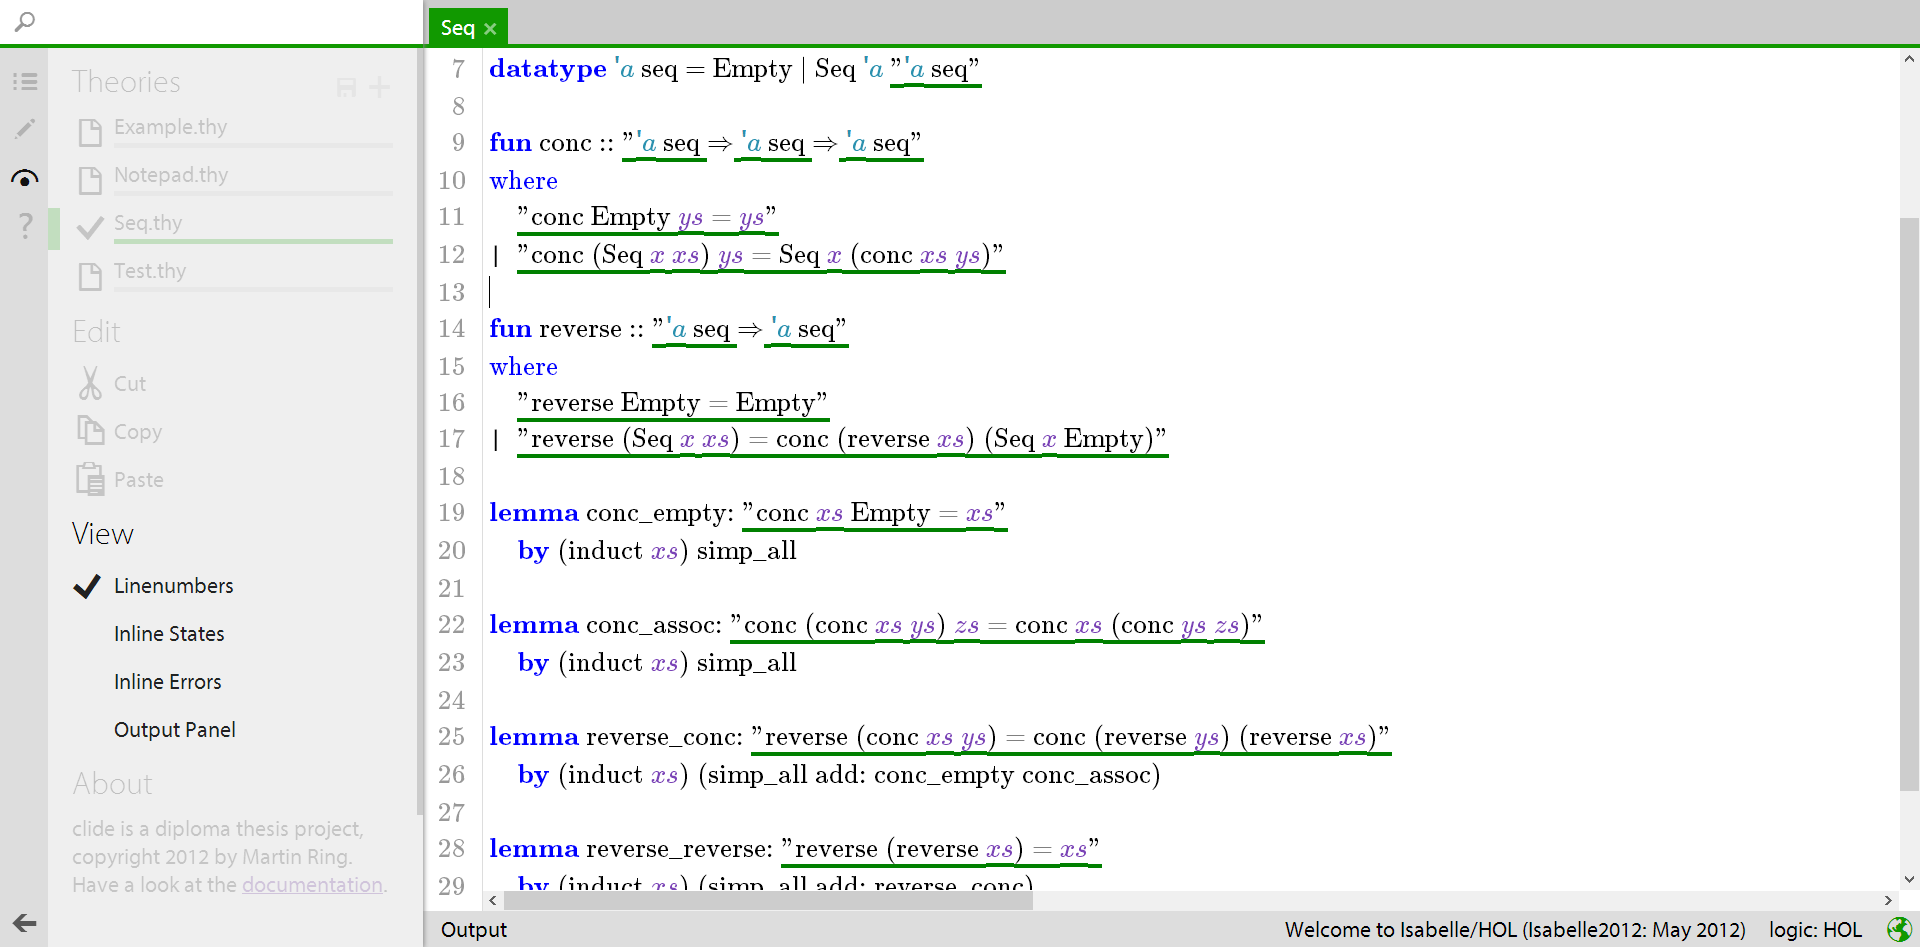
\includegraphics[width=\linewidth]{images/sssyntax}
  \caption{Serverseitiges Syntax-Highlighting}
  \label{fig:sssyntax}
\end{figure}

Im Browser wird eine Liste der Kommandos im Quelltext verwaltet, welche der Server ständig durch
Nachrichten aktualisiert. Dafür wurde auf dem Client in \texttt{isabelle.coffee} ein Backbone-Modell
für die Repräsentation der relevanten Daten von Kommandos (\texttt{Command}) entworfen.

\begin{lstlisting}[language=coffee]
  class Command extends Backbone.Model
    ...

  class Commands extends Backbone.Collection
    model: Command    
    getCommandAt: (line) => 
      ...
    getTokenAt: (line,column) =>
      ...
\end{lstlisting}

Das \texttt{Commands}-Modell dient der Verwaltung der Liste und ist eine Backbone-Collection, die
den Vorteil bietet, dass sie über Callbacks für Modifikationen (\texttt{on 'remove'}, \texttt{on
'add'}, ...) verfügt und somit das Markup im Editor bei Bedarf aufgefrischt werden kann.

Die Klasse \texttt{Session} in \texttt{isabelle.coffee} dient hier als Schnittstelle für den Server
und wird über einen ScalaConnector (Abschnitt\,\ref{sec:jsc}) mit dem WebSocket verbunden.

Auf Serverseite existiert ebenfalls eine Klasse \texttt{Session} in \texttt{Session.scala} welche
wiederum das Gegenstück darstellt und über den \texttt{JSConnector} verbunden ist.

Wenn nach einer Änderung am Dokument neue Kommandos erkannt werden bzw. sich Kommandos verändert
haben oder Kommandos wegfallen, wird dies über den Nachrichtenkanal \texttt{Session.commandsChanged}
in Erfahrung gebracht und die Information aufbereitet.

\begin{lstlisting}
session.commands_changed += { change =>
  change.nodes.foreach { node =>
    delayedLoad(node)
    val snap = session.snapshot(node, Nil)
    val status = Protocol.node_status(snap.state, snap.version, snap.node)      
    js.ignore.status( ... )      
    for {
      doc <- docs.get(node)        
    } {        
      js.ignore.states(node.theory, MarkupTree.getStates(snap, doc.buffer.ranges))
      val cmds = snap.node.commands.map(_.id)
      doc.commands.keys.foreach { id =>
        if (!cmds.contains(id)) {
          doc.commands.remove(id)
          js.ignore.removeCommand(node.toString, id)
        }
      }
    }       
  }
  change.commands.foreach(pushCommand)    
}
\end{lstlisting}

Im \texttt{RemoteDocumentModel} wird dafür eine synchrone Repräsentation der Kommandos verwaltet.
Sollte ein Kommando hier nicht mehr existieren, wird es über die Nachricht
\texttt{js.ignore.removeCommand(...)} im Browser entfernt, damit die Ressourcen dort freigegeben
werden können bzw. Syntaxmarkierungen aus dem Dokument entfernt werden können.

Über \texttt{pushCommand} werden alle veränderten Kommandos verarbeitet. Wenn sich dann die
gefilterten, relevanten Informationen von denen im \texttt{RemoteDocumentModel} unterscheiden,
werden die neuen Informationen dort an den Client weitergeleitet. In diesen Informationen enthalten
sind:

\begin{itemize}
  \item Token aus der Inneren Syntax,
  \item Token mit Typinformationen,
  \item Fehlerhafte Token mit den zugehörigen Fehlermeldungen sowie
  \item der Beweiszustand des Kommandos.
\end{itemize}

Weil die verschiedenen Tokenmengen nicht zwingender Weise disjunkt sind, werden die Vereinigungen
der jeweiligen Informationen betrachtet und Überschneidungen gegebenenfalls aufgebrochen (in
\texttt{MarkupTree.scala}).

Auf dem Client werden von den Editoren (\texttt{Editor.coffee}) die Callbacks der Kommandoliste der
jeweils angeschlossenen Theorie verarbeitet und dann die Informationen in die Darstellung
integriert.

\begin{lstlisting}
includeCommand: (cmd) => 
  if cmd.get('version') is @model.get('currentVersion') then @cm.operation =>
    unless cmd.get('registered')      
      cmd.on 'remove', (cmd) => if cmd?
        for m in cmd.get 'markup'
          m.clear()
        wid = cmd.get('widget')
        if wid?
          @cm.removeLineWidget(wid)
      cmd.set registered: true

    # add line widget
    @addCommandWidget(cmd)

    # mark Stuff
    old = cmd.get('markup')
    if old?
      for m in old
        m.clear()
    range  = cmd.get 'range'
    length = range.end - range.start
    marks = []
    for line, i in cmd.get 'tokens'
      l = i + range.start
      p = 0
      for tk in line
        from = 
          line: l
          ch: p
        p += tk.value.length
        unless (tk.type is "text" or tk.type is "")
          to =
            line: l
            ch: p              
          marks.push(@cm.markText from,to,
            className: "cm-#{tk.type.replace(/\./g,' cm-')}"
            tooltip: tk.tooltip
            __isabelle: true)
    cmd.set((markup: marks),(silent: true))
\end{lstlisting}



\section{Substitution von Symbolen}

Die in den vorherigen Abschnitten beschriebenen Tokenklassen werden verwendet, um Symbole direkt im
Quelltext zu substituieren. Da CodeMirror glücklicherweise seit Version 3.0, welche gegen Ende der
Bearbeitungszeit dieser Diplomarbeit veröffentlicht wurde die Möglichkeit bietet, Textstellen durch
HTML-Widgets zu ersetzten, konnte ein vorheriger serverseitiger Ansatz, der von Natur aus recht
fehleranfällig war, verworfen werden.

\begin{figure}[ht]
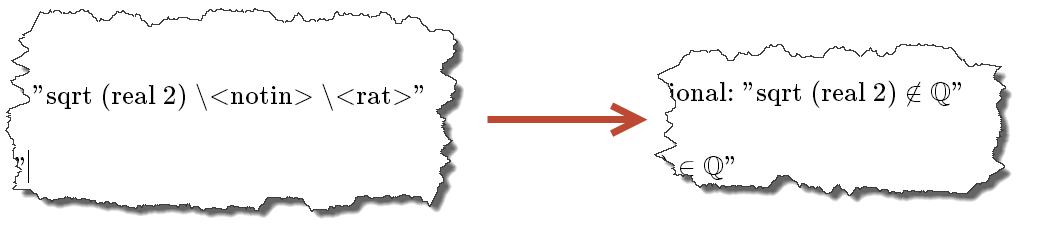
\includegraphics[width=\linewidth]{images/subst}
  \caption{Substitution von Symbolen}
  \label{fig:subst}
\end{figure}

Die grundsätzliche Idee bei der Symbol-Substitution ist es, den eigentlichen Isabelle-Quelltext auf
Clientseite unverändert zu lassen und nur die Visualisierung anzupassen. Die Substitution findet in
\texttt{/app/assets/javascripts/rjs/editor.coffee} statt.

Hierfür werden während des Ladens eines Dokuments zunächst alle Vorkommen von Spezialsymbolen
ersetzt. Dafür bedienen wir uns des CodeMirror Plugins \texttt{SearchCursor}, das es erlaubt den
Text mit regulären Ausdrücken effizient zu durchsuchen.

\begin{lstlisting}[language=coffee]
cursor = @cm.getSearchCursor(special)
while cursor.findNext()
  sym = symbols[cursor.pos.match[0]]
  if sym?
    from = cursor.from()
    to   = cursor.to()
    @cm.markText from, to,
      replacedWith: sym(),
      clearOnEnter: false    
\end{lstlisting}

Im laufenden Betrieb werden dann bei jeder Veränderung die Tokenklassen an den veränderten
Positionen betrachtet, um zu entscheiden, ob es sich um Spezialsymbole handelt.

Dafür wird das \texttt{onchange}-Callback der CodeMirror-Instanz implementiert. Wir verwenden an
dieser Stelle \texttt{.operation} um die gesamte Operation auszuführen, bevor die Visualisierung
angepasst wird, dadurch wird die Ausführungsgeschwindigkeit drastisch erhöht. Zudem stellen wir
sicher, dass keine Selektion vorliegt, da in diesem Fall zunächst keine Ersetzungen Stattfinden
sollen bis die Selektion wieder aufgehoben wurde.

\begin{lstlisting}[language=coffee]
@cm.on 'change', (editor,change) => editor.operation => unless editor.somethingSelected()
  ...
\end{lstlisting}

Nun löschen wir alle an dieser Stelle zuvor eingeführten Substitutionen (durch die Eingabe kann sich
das zu substituierende Zeichen verändert haben). Da wir \texttt{CodeMirror.operation} verwenden, ist
diese Aktion relativ performant.

\begin{lstlisting}[language=coffee]
pos   = change.to
token = editor.getTokenAt(pos)          
marks = editor.findMarksAt(pos)
mark.clear() if mark.__special for mark in marks 
\end{lstlisting}

Wenn es sich bei dem aktuellen Token nun um ein spezielles Zeichen handelt, dann wird es mit Hilfe
des CoffeeScript Moduls \texttt{symbols}, welches über RequireJS importiert wurde zu einem Widget
übersetzt, das dann als Textsubstitution eingesetzt werden kann.

\begin{lstlisting}[language=coffee]
    if token.type? and (token.type.match(/special|symbol|control|sub|sup|bold/))
      wid = symbols[token.string]
      if wid?
        @cm.markText from,to,          
          replacedWith: wid(token.type)
          clearOnEnter: false
          __special:    true
\end{lstlisting}

Das \texttt{symbols}-Modul wurde aus der Datei \texttt{/etc/symbols} in der Isabelle Plattform
abgeleitet. Zusätzlich wurden Informationen über den zu verwendenden \LaTeX-Font (Caligraphic,
Fraktur, AMS, ...) für jedes Symbol manuell eingearbeitet.

\begin{figure}[ht]
\centering
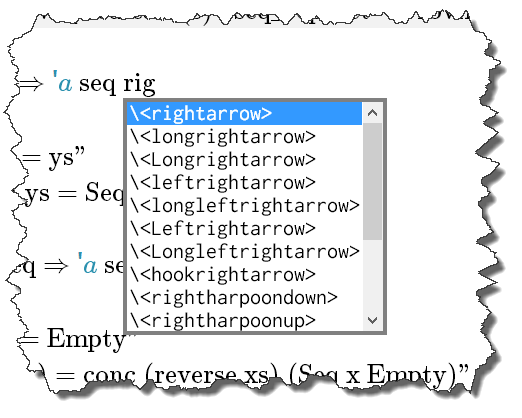
\includegraphics[width=0.5\linewidth]{images/completion}
  \caption{Vervollständigung von Symbolsubstitutionen}
  \label{fig:subst}
\end{figure}


\section{Modale Dialoge}

Um die Funktionsweise von \texttt{Backbone.View} und das Zusammenspiel mit dem ScalaConnector zu
illustrieren, betrachten wir an dieser Stelle ein einfaches Beispiel. An manchen Stellen in der
Anwendung ist es notwendig, den Benutzer mit modalen Dialogen zur Beantwortung einer Frage
aufzufordern. Hierfür wurde das Modul \texttt{Dialog.coffee} entworfen.

\begin{lstlisting}
define ->
  class Dialog extends Backbone.View
\end{lstlisting}

Beim Initialisieren wird abhängig von den übergebenen Optionen die \acr{ui} aufgebaut. Mögliche
Optionen sind dabei

\begin{itemize}
  \item ein String \texttt{title} um eine Überschrift zu erzeugen,
  \item ein String \texttt{message} um die eigentliche Nachrich zu spezifizieren,
  \item ein Array \texttt{buttons} um festzulegen, welche Buttons angezeigt werden soll,
  \item \texttt{defaultAction} um den Standard Button festzulegen, welche ausgelöst wird, wenn der
  Nutzer einfach Enter drückt,
  \item ein String \texttt{defaultText}, welcher zum Festlegen eines \texttt{input[type=text]} 
  Controls sowie eines eventuellen vorgegebenen Inhalts dient sowie
  \item ein Callback \texttt{done} um das Ergebnis der Nutzereingabe zu verarbeiten.
\end{itemize}

Die Optionen können weggelassen werden, sodass auf Standardwerte zurückgegriffen wird, bzw. der
Titel oder die Nachricht weggelassen werden.

Wenn ein Button geklickt wird oder Enter gedrückt wird, wird die \texttt{exit}-Funktion aufgerufen,
welche den Dialog aus dem \acr{dom} entfernt und das \texttt{done}-Callback aufruft. \texttt{text}
ist dabei \texttt{undefined}, wenn kein Input-Control erzeugt wurde.

\begin{lstlisting}
    exit: (action) => () =>
      text = @$('input').val()
      @$el.remove()
      if @options.done then @options.done
        action: action
        text: text
\end{lstlisting}

Nun können wir beispielsweise als Aktion eines Kontextmenüeintrages \glqq Löschen\grqq zunächst
einen Modalen Dialog erstellen um sicherzugehen, dass die Aktion vom Nutzer gewollt ist.

\begin{lstlisting}
  menu.show(e.pageX,e.pageY,[
      text: 'Delete'
      command: ->
        new Dialog
          title: "Delete Project"
          message: "Do you really want to delete project '#{$(elem).data('name')}'?"
          buttons: ['Yes','No']
          defaultAction: 'Yes'
          done: (e) => if e.action is 'Yes' then deleteProject(user,$(elem).data('name'))                  
    ])
\end{lstlisting}

Das Spannende daran ist nun, dass es möglich ist, diese Dialoge über den \texttt{JsConnector} bzw.
den \texttt{ScalaConnector} vom Server aus zu erzeugen und zu nutzen. So kann der Server bei Bedarf
über \texttt{js.sync} eine blockierende Frage auf dem Client stellen und erst nach der Antwort des
Nutzers fortfahren, genauso wie es in Desktopanwendungen über Messageboxen üblich ist.

\begin{figure}[ht]
\centering
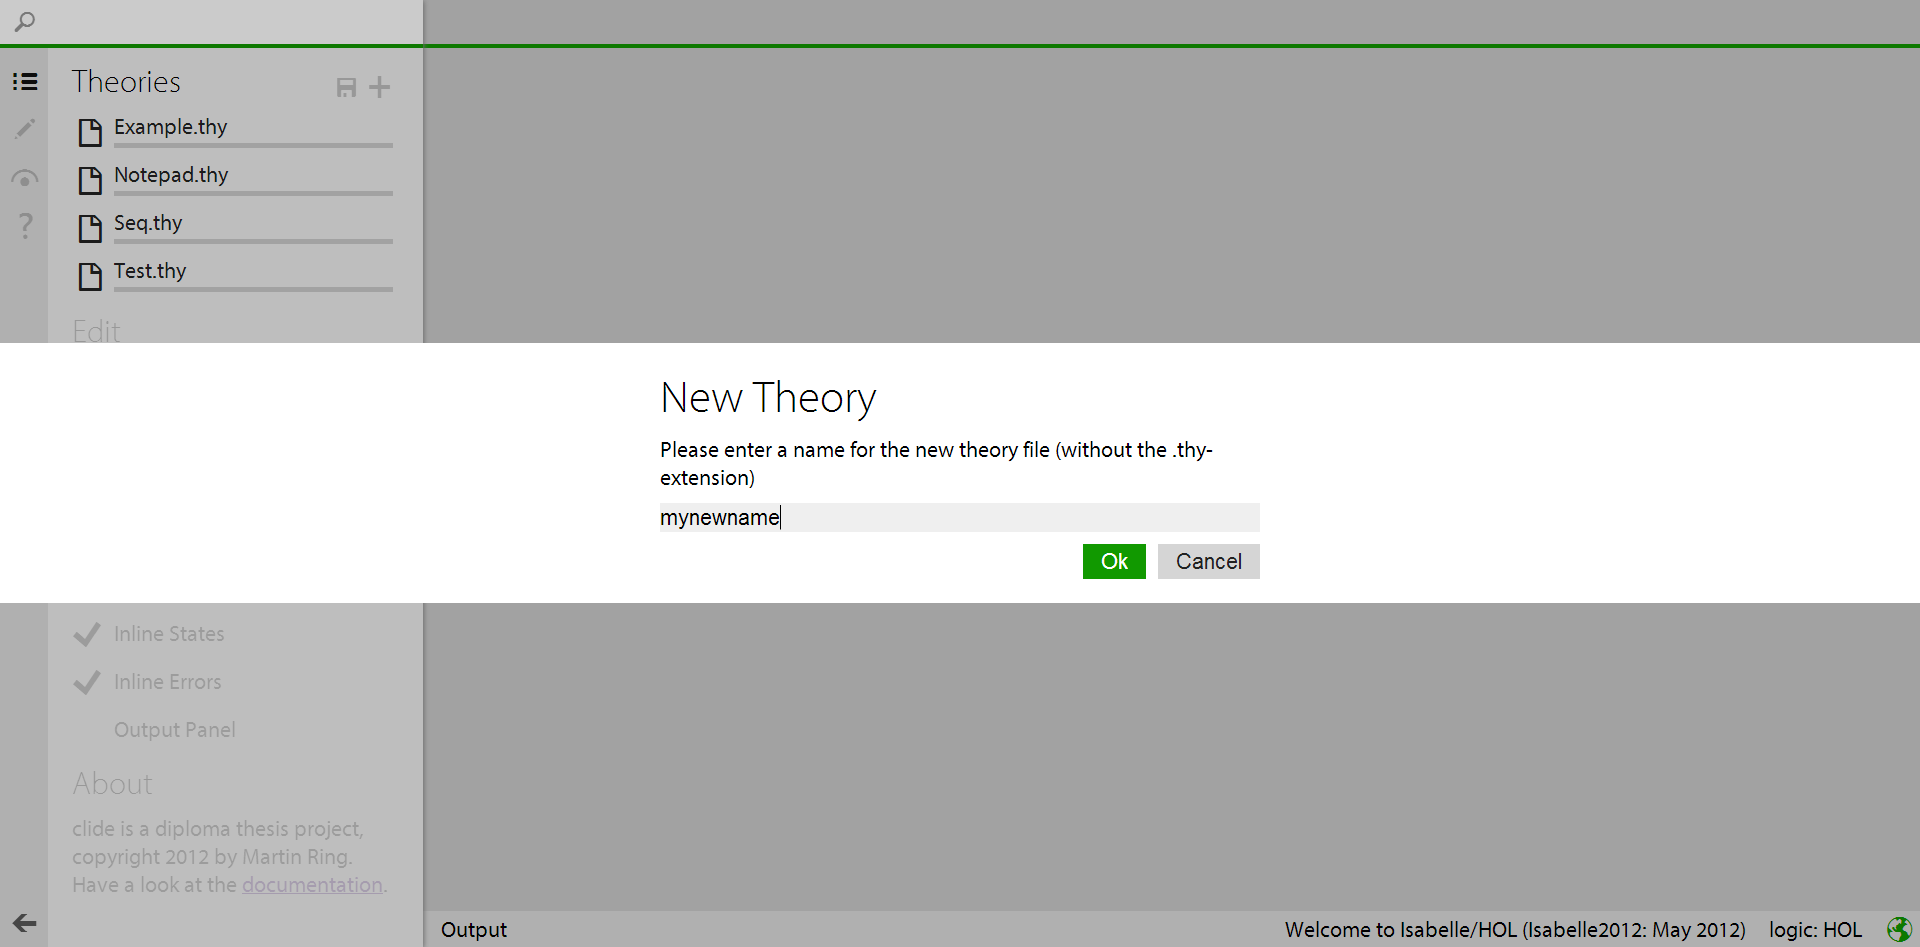
\includegraphics[width=\linewidth]{images/screen-dialog}
  \caption{Ein modaler Dialog}
  \label{fig:dialog}
\end{figure}
